% figure: 现控强化3-24-降维观测反馈结构图.png
\documentclass[border=12pt]{standalone}
\usepackage{fontspec}
\setmainfont{Cambria}
\usepackage{unicode-math}
\setmathfont{Cambria Math}
\usepackage{tikz}
\usetikzlibrary{arrows.meta,calc}
\begin{document}
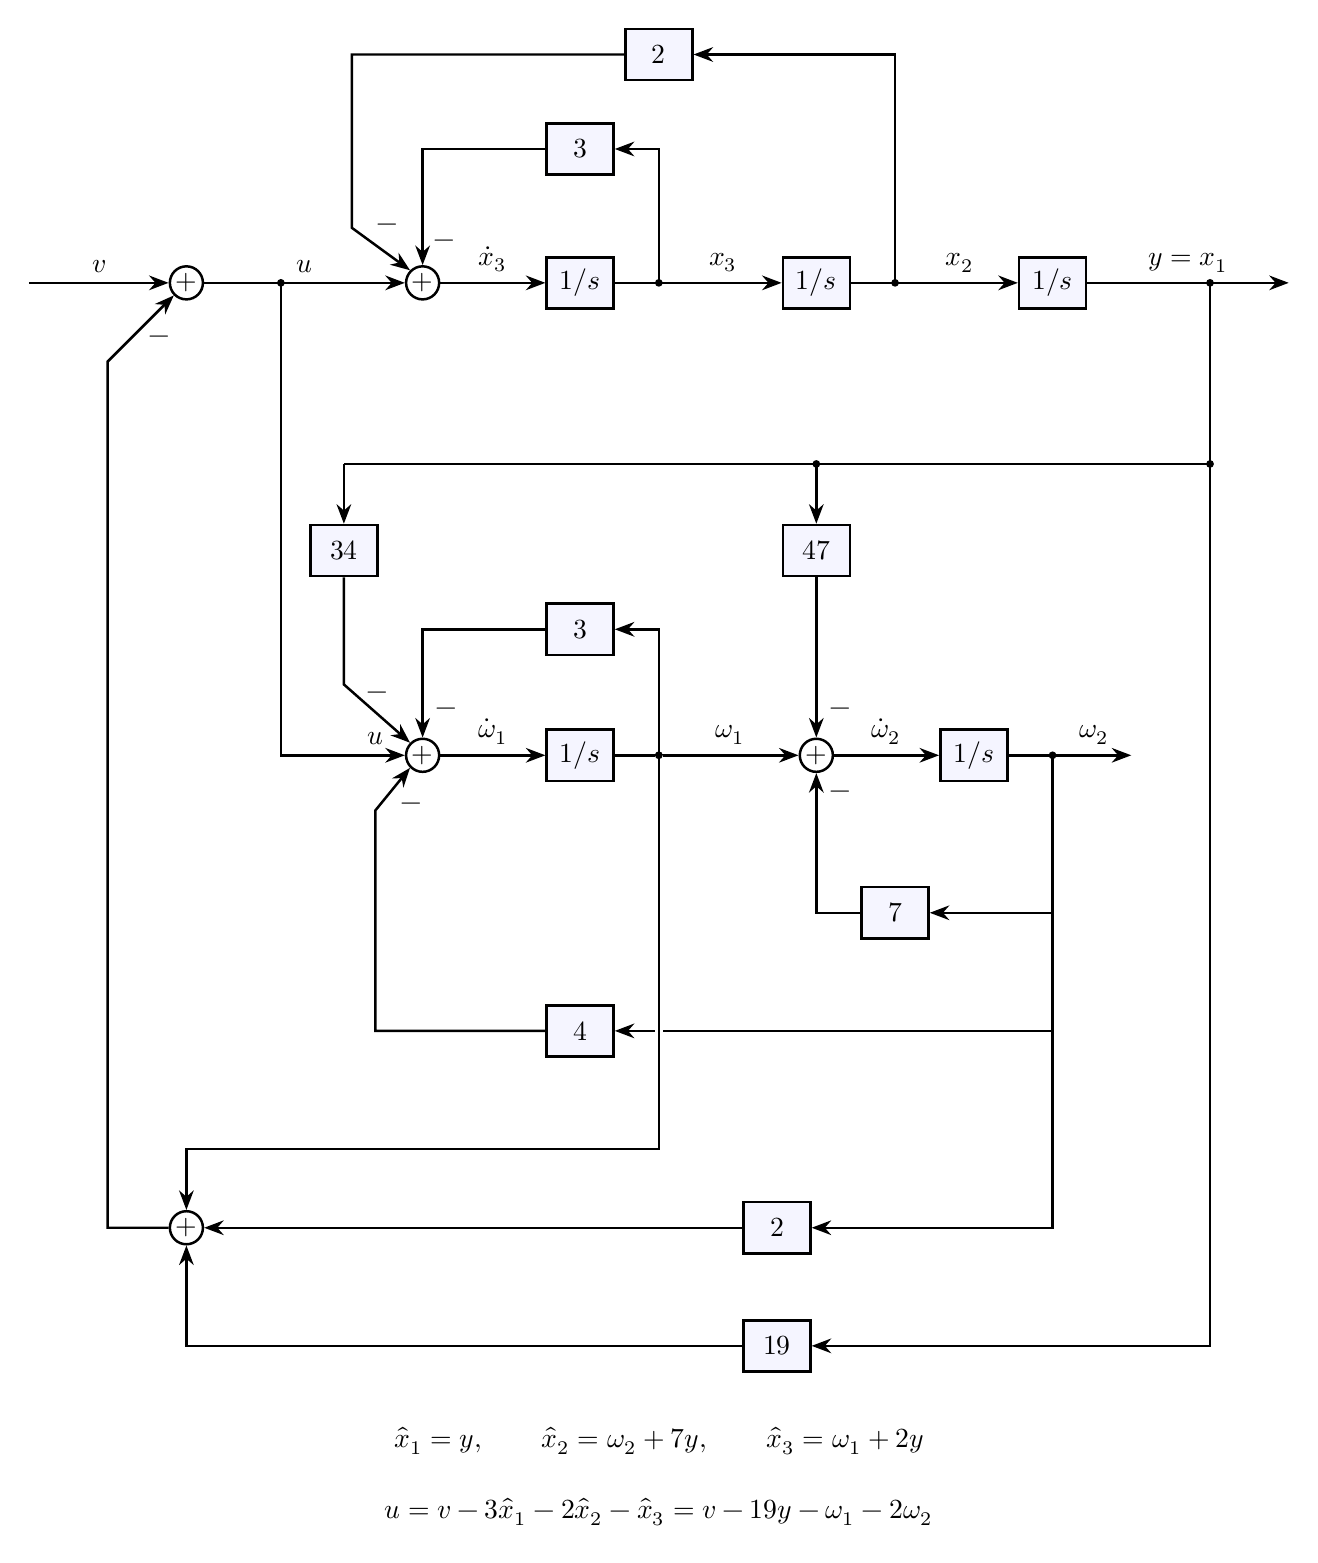
\begin{tikzpicture}[>=Stealth,line width=.9pt,
 b/.style={draw,minimum width=.85cm,minimum height=.65cm,fill=blue!4},
 s/.style={draw,circle,minimum size=.42cm,inner sep=0pt},
 cross/.style={preaction={draw=white,line width=3pt}}]
% Plant: x3dot = u - 3 x3 - 2 x2, x2dot = x3, x1dot = x2.
\node[s] (su) at (0,0) {$+$};
\node[s] (sp) at (3,0) {$+$};
\node[b] (p3) at (5,0) {$1/s$};
\node[b] (p2) at (8,0) {$1/s$};
\node[b] (p1) at (11,0) {$1/s$};
\node[b] (a3) at (5,1.7) {$3$};
\node[b] (a2) at (6,2.9) {$2$};
\draw[->] (-2,0) -- node[above] {$v$} (su);
\draw[->] (su) -- node[above] {$u$} (sp);
\draw[->] (sp) -- node[above] {$\dot x_3$} (p3);
\draw[->] (p3) -- node[above,pos=.65] {$x_3$} (p2);
\draw[->] (p2) -- node[above,pos=.65] {$x_2$} (p1);
\draw[->] (p1) -- node[above] {$y=x_1$} (14,0);
\fill (6,0) circle(1.4pt);
\fill (9,0) circle(1.4pt);
\fill (13,0) circle(1.4pt);
\draw[->] (6,0) |- (a3.east);
\draw[->] (a3.west) -| (sp.north);
\node at (3.28,.5) {$-$};
\draw[->] (9,0) |- (a2.east);
\draw[->] (a2.west) -- (2.1,2.9) -- (2.1,.7) -- (sp.north west);
\node at (2.55,.7) {$-$};
% Two scalar observer integrators, with known input u retained explicitly.
\node[s] (s1) at (3,-6) {$+$};
\node[b] (o1) at (5,-6) {$1/s$};
\node[s] (s2) at (8,-6) {$+$};
\node[b] (o2) at (10,-6) {$1/s$};
\node[b] (f3) at (5,-4.4) {$3$};
\node[b] (f7) at (9,-8) {$7$};
\node[b] (f4) at (5,-9.5) {$4$};
\node[b] (l34) at (2,-3.4) {$34$};
\node[b] (l47) at (8,-3.4) {$47$};
\fill (1.2,0) circle(1.4pt);
\draw[->] (1.2,0) |- node[pos=.88,above] {$u$} (s1.west);
\draw[->] (s1) -- node[above] {$\dot\omega_1$} (o1);
\draw[->] (o1) -- node[above,pos=.63] {$\omega_1$} (s2);
\draw[->] (s2) -- node[above] {$\dot\omega_2$} (o2);
\draw[->] (o2) -- node[above,pos=.7] {$\omega_2$} (12,-6);
\fill (6,-6) circle(1.4pt);
\fill (11,-6) circle(1.4pt);
\draw[->] (6,-6) |- (f3.east);
\draw[->] (f3.west) -| (s1.north);
\node at (3.3,-5.45) {$-$};
\draw[->] (11,-6) |- (f7.east);
\draw[->] (f7.west) -| (s2.south);
\node at (8.3,-6.5) {$-$};
\draw[->] (11,-6) |- (f4.east);
\draw[->] (f4.west) -- (2.4,-9.5) -- (2.4,-6.7) -- (s1.south west);
\node at (2.85,-6.65) {$-$};
% One output bus supplies the two injection gains and the feedback gain 19.
\draw (13,0) -- (13,-2.3) -- (2,-2.3);
\fill (8,-2.3) circle(1.4pt);
\fill (13,-2.3) circle(1.4pt);
\draw[->] (2,-2.3) -- (l34.north);
\draw[->] (8,-2.3) -- (l47.north);
\draw[->] (l34.south) -- (2,-5.1) -- (s1.north west);
\node at (2.42,-5.25) {$-$};
\draw[->] (l47.south) -- (s2.north);
\node at (8.3,-5.45) {$-$};
% u = v - (19 y + omega1 + 2 omega2).
\node[s] (sk) at (0,-12) {$+$};
\node[b] (k2) at (7.5,-12) {$2$};
\node[b] (k19) at (7.5,-13.5) {$19$};
\draw[->,cross] (6,-6) -- (6,-11) -- (0,-11) -- (sk.north);
\fill (6,-6) circle(1.4pt);
\draw[->] (11,-9.5) -- (11,-12) -- (k2.east);
\draw[->] (k2.west) -- (sk.east);
\draw[->] (13,-2.3) -- (13,-13.5) -- (k19.east);
\draw[->] (k19.west) -- (0,-13.5) -- (sk.south);
\draw[->] (sk.west) -- (-1,-12) -- (-1,-1) -- (su.south west);
\node at (-.35,-.72) {$-$};
\node[anchor=north] at (6,-14.4) {$\hat x_1=y,\qquad \hat x_2=\omega_2+7y,\qquad \hat x_3=\omega_1+2y$};
\node[anchor=north] at (6,-15.3) {$u=v-3\hat x_1-2\hat x_2-\hat x_3=v-19y-\omega_1-2\omega_2$};
\end{tikzpicture}
\end{document}
